%*******************************************************************************
%****************************** Second Chapter *********************************
%*******************************************************************************

\chapter{Related Work}
\label{chapter_related}

\ifpdf
    \graphicspath{{Chapter2/Figs/Raster/}{Chapter2/Figs/PDF/}{Chapter2/Figs/}}
\else
    \graphicspath{{Chapter2/Figs/Vector/}{Chapter2/Figs/}}
\fi

This chapter reviews the related work relevant for this thesis. Since there are many different related work areas that all have their relevance to this thesis, this chapter is divided into different sections dealing with each of them in turn. First section \ref{sec_basicDefinitions} introduces and defines basic the basic terminology that will be used in this thesis. Subsequently section \ref{sec_streamMining} gives a broad overview over the rather general area of mining data streams with a focus on prediction. Finally section \ref{sec_episodes} introduces the concept of episodes and summarizes different episode mining approaches.

\section{Basic Definitions and Terminology}
\label{sec_basicDefinitions}
This section introduces relevant definitions and terminology that was introduced in previous work and will be used in this thesis.

\subsection{Event Processing Terminology}
The basic event terminology in this subsection is paraphrased from the event processing glossary created by the Event Processing Technical Society \cite{luckham2011epts}. Note that some of the definitions may be slightly altered or simplified. This is due to the fact that the event processing technical society uses these terms for a very general description of event processing and event processing architectures and thus some original definitions are more complex than what is needed in this thesis. The definitions given here aim to establish a clear terminology for this thesis.

\begin{mydef}
\textbf{Event} An event is either something that is happening in the real world or in the context of computer science an object that represents a real world event and records its properties. The latter can also be referred to as an event object or an event tuple. Note that the term is overloaded, but the context usually gives a clear indication of what is meant.
\end{mydef}

The event processing society claims that the context usually solves the ambiguity in the above definition. Since this may not always be the case we will only use the term \textit{event} in this thesis to refer to event objects unless it is otherwise specified.

\begin{mydef}
\textbf{Simple Event} A simple event is an event that is not viewed as summarizing, representing, or denoting a set of other events. Sometimes also referred to as a basic events.
\end{mydef}

These two definitions can sometimes cause confusion. It is important to note that the term event is the most general term, since it can refer to any kind of event, be it simple, derived or complex (see definitions \ref{def_derivedEvent} and \ref{def_complexEvent}). A simple event however is the most basic form of an event and often the ingredient for the creation of more complex events:
Given simple events it is possible to derive events from those or the absence of those. For example the absence measurement events of a sensor could be used to derive the event of that very same sensor becoming defect. These events are called derived events:

\begin{mydef}
\label{def_derivedEvent}
\textbf{Derived Event} A derived event or synthesized event is an event that is generated according to some method or based on some reasoning process.
\end{mydef}

It is also possible to combine multiple simple events to form what we refer to as complex events:

\begin{mydef}
\label{def_complexEvent}
\textbf{Complex Event} A complex event is a derived event that is created by combining other events. The events can be combined by using certain operators, for example disjunction, conjunction or sequence. An example would be $(A \land B) \rightarrow C$ (event A and B in any order followed by event C).
\end{mydef}

This is a very broad definition of complex events. The choice of allowed operators strongly impacts the expressiveness of complex events. A specific kind of complex events are episodes (see section \ref{sec_episodes}), which will be the main focus of this thesis.
The next notion that needs to be considered is that each individual event normally belongs to a certain class of events, which we refer to as the event type:

\begin{mydef}
\textbf{Event type} The event type, sometimes also referred to as event class, event definition, or event schema is a label that identifies events as members of an event class.
\end{mydef}

Another important term that was not explicitly defined in the event processing glossary, but is very relevant to the topic at hand is the notion of a type alphabet:

\begin{mydef}
\textbf{Type Alphabet} The type alphabet, often simply called the event alphabet, is the set of all possible event types that can occur in the observed system.
\end{mydef}

Event alphabets are often implicitly defined when mining frequent itemsets, patterns or episodes.
So far we have looked at events without considering the scenario we are most interested in which are event streams. To do so we need the notion of timestamps:

\begin{mydef}
\textbf{Timestamp} A time value of an event indicating its creation or arrival time.
\end{mydef}

Given that we can define an event stream:

\begin{mydef}
\textbf{Event Stream} An event stream is an ordered sequence of events, usually ordered by the event timings.
\end{mydef}

Note that this rather broad definition of an event stream does not assume anything about the kind of event that is contained in it. A stream can contain very basic forms of events (simple events) but can also be made up out of derived events or even complex events. Also other properties for example that the stream is constantly updating (new events coming in) are not considered yet.


\section{Data Stream Mining}
As already mentioned in the introduction data streams present a challenge to data miners in many ways. This section aims to give both a general overview over the broad research area of mining data stream as well as specifically cover the related topics of forecasting and stock market prediction.

 %Section \ref{subsec_patternMining} gives an overview on classical pattern mining and frequent itemset mining approaches. Section \ref{subsec_regression} continues with an outline of the state of the art classification and regression approaches after which section \ref{subsec_prediction} will take a closer look on time series prediction with a focus on financial data and stock market forecasting.
%Section \ref{subsec_dataStreamProcessing} then introduces related work in the very broad research area of processing and mining data streams. Afterwards section \ref{subsec_eventProcessing} presents the research area of general event processing with a focus on the mining of complex events and episodes. Finally section \ref{subsec_semanticWeb} finishes with an overview over the most relevant work (with respect to this thesis) in the research area of the semantic web.

%\subsection{Pattern Mining}
%\label{subsec_patternMining}
%Of all the fields related to this thesis basic pattern mining is arguably the most well researched and widely used related research area. First to mention are of course the standard pattern mining algorithms for frequent itemsets \cite{han2007frequent}. The authors of this paper nicely summarize different approaches, which either use candidate generation and the apriori-principle or pattern growth strategies. Problematic with the original Apriori-Algorithm is of course that while the apriori-principle helps to prune the candidate generation, its runtime can still be exponential. On top of that it requires multiple passes over the database, which is something that can be impossible given large data streams. These general pattern mining algorithms have of course already been modified or improved for more specific purposes. For example event data logs have been used to build predictive models that search for patterns that predict critical events in the log file \cite{chen2014pattern}. \newline
%A rather large subfield of pattern mining is the field of (business) process mining. This particular domain usually evaluates log-files of (business) applications that log sequences of events. These logs can be mined to satisfy many different information needs, for example clustering \cite{vaarandi2015logcluster} or process models \cite{priyadharshini2016analysis}.
%Another approach in the field of business logs and process mining is outlier and anomaly detection \cite{sureka2015kernel}. The authors use the length of the longest common subsequence between event sequences as a distance measure to find unusual patterns of events. This field of interest is especially interesting since there are a lot of business applications, some of which use legacy software, whose behaviour is at times unclear or error-prone. Mining underlying business models or unusual behavior can help identify errors. \newline
%A subfield of pattern mining that is especially relevant for this thesis is sequential pattern mining. Comprehensive overviews are given by Slimani et al. \cite{slimani2013sequential} as well as Zhao at al. \cite{zhao2003sequential}.

\subsection{Data Stream Mining Taxonomy}
\label{subsec_dataStreamMiningTaxonomy}
Many research areas in classical data mining are also of interest when processing streams. As already mentioned in the introduction however, data streams impose severe restrictions on the algorithms, such them having to use only one pass over the data and that they should be incremental. Normally data mining algorithms for the classical scenario in which the underlying data is a static database or even a data-set that fits into main memory have these properties. Thus the algorithms need to be modified and often approximations have to be made. A comprehensive basic overview over the application of different data mining tasks and how they can be applied to streams was comprised by Gaber et. al. \cite{gaber2005mining}. A taxonomy that follows the basic structure of the overview by Gaber et. al. is visualized in figure \ref{fig_streamMiningTaxonomy}.

\begin{figure}[h]
	\centering
  	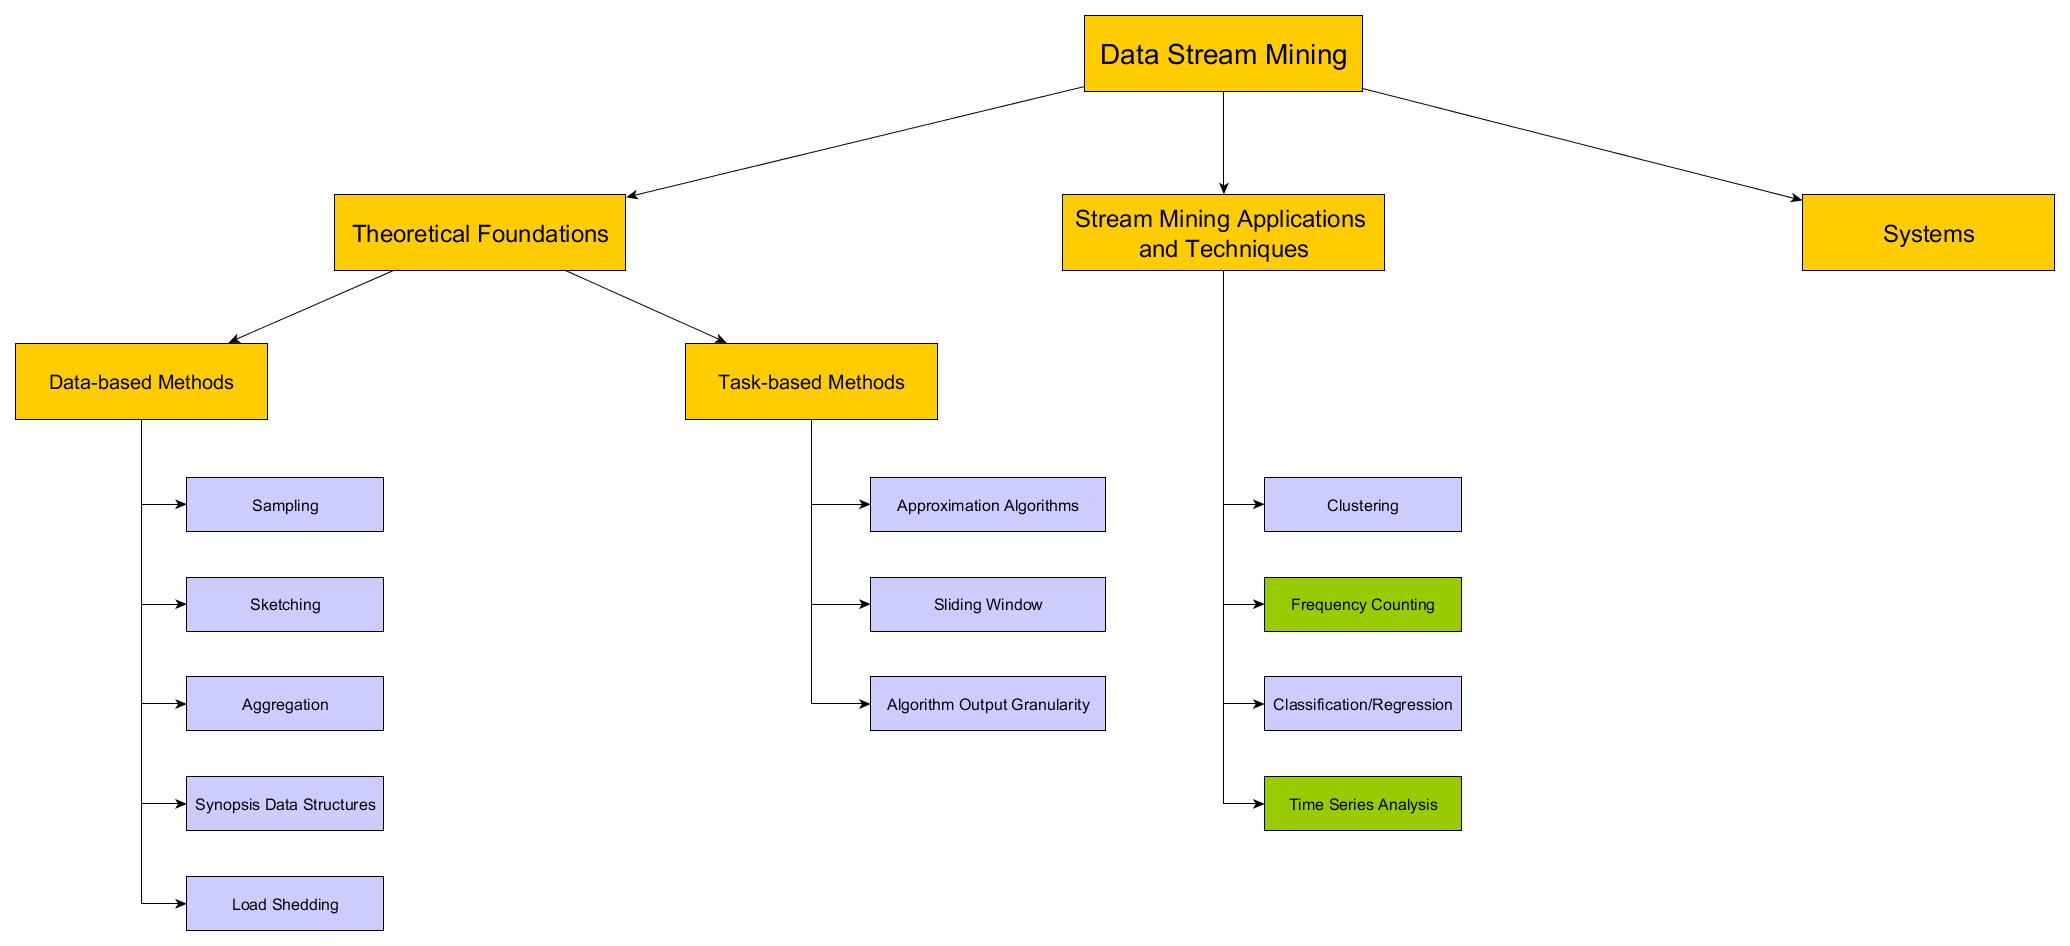
\includegraphics[width=\textwidth]{streamMiningTaxonomy}
	\caption{A taxonomy of the research areas of data stream mining. The subcategories that are marked green are the categories to which this thesis will make contributions.}
	\label{fig_streamMiningTaxonomy}
\end{figure}

As can be seen in the figure the state of the art in data stream mining can be roughly divided into three basic parts:

\begin{enumerate}
	\item Theoretical Foundations
	\item Mining Techniques and Applications
	\item Systems
\end{enumerate}

The theoretical foundations contain general approaches on how to deal with the issues of data streams. There is a distinction between data-based techniques and task-based techniques. Data-based techniques aim to reduce the data being processed or apply transformations on the data stream, while task-based techniques are modifications of existing techniques to meet the requirements for time and space. The subcategories of data-based techniques are:

\begin{itemize}
	\item \textbf{Sampling:} The idea of sampling is basically the same as in statistics. Instead of processing the whole stream, only a subset of the stream is looked at. Due to the unknown size of the stream, sampling methods are more complex than in static systems like databases (TODO: extra reference). 
	\item \textbf{Load Shedding:} Load shedding is similar to sampling in that it simply drops certain incoming data without processing it, however load shedding is a dynamic approach that is only applied if needed, for example if there are volume spikes (large amounts of data coming in suddenly). Thus in contrast to sampling, which is applied over the whole lifetime of the stream, load shedding is a more reactionary strategy \cite{babcock2003load}.
	\item \textbf{Sketching:} When we speak of sketching we refer to the process of building a summary of the data stream that only uses very little memory compared to the whole stream. Examples of this are the so-called frequency moments \cite{babcock2002models}
	\item \textbf{Synopsis Data Structures:} Synopsis data structures summarize the stream in data structures that are then used to approximately answer queries. TODO: difference between synopsis and sketches.
	\item \textbf{Aggregation:} Aggregation is mainly useful when statistical measures are to be computed over a stream. TODO: reference?
\end{itemize}

The task-based techniques mentioned by the authors are:

\begin{itemize}
	\item \textbf{Approximation Algorithms:} Approximation algorithms are common for hard problems (such as NP-complete problems) but also many classic data-mining problems can be solved on data streams using approximate variants of the original algorithms. A commonly cited example are approxiamtion algorithms for the mining frequent items or itemsets, such as the sticky sampling or the lossy counting algorithm \cite{manku2002approximate}.
	\item \textbf{Sliding Window:} The usage of sliding windows over the data streams is common when the user is only interested in the most recent events as opposed to the complete history. The main challenge here is to construct algorithms that work with the incremental updates that happen whenever new data arrives (the window slides forward). (TODO: cite something)
	\item \textbf{Algorithm Output Granularity:} The term algorithm output granularity refers to the strategy of dynamically reacting to the available memory and fluctuating data rates. The basic idea is to mine the incoming data stream as long as possible (normally until the device runs out of memory). If this happens the generated knowledge structures are merged and summarized in order to free up memory and continue the mining. 
\end{itemize}

The second category contains the actual mining techniques and applications, which are well known from classical data mining:

\begin{itemize}
	\item \textbf{Clustering} TODO
	\item \textbf{Classification and Regression} Classification and regression in evolving data streams presents the additional challenges of concept drift, which means that the underlying class distribution may change, which will make the originally built model invalid over time. TODO: cite stuff here
	\item \textbf{Frequency Counting} TODO
	\item \textbf{Time Series Analysis} TODO
\end{itemize}

The last category in the taxonomy is less focused on research issues and conceptual or algorithmic problems but instead lists the existing data stream processing systems (to that date). Since that is less relevant to this thesis we do not mention or describe existing systems but instead refer the interested reader to the original paper by Gaber et. al. \cite{gaber2005mining}. \newline
TODO: Note that the paper by Gaber et. al. was published in 2005, so quite a lot of work has been done since then, which means that these are obviously not present in their overview. An example for this is the popular hadoup system (TODO: verify that). However the established taxonomy is still very useful, since it brings structure to the large field of data stream mining. \newline
As visualized in figure \ref{fig_streamMiningTaxonomy} this thesis mainly deals with the subtopics of time series data and pattern mining, which is why these two areas of work will now be inspected more closely in the next subsections

\subsection{Pattern Mining in Data Streams}
TODO: Adrians Überblicksgrafik

\subsection{Time Series Analysis in Data Streams}
Before diving deeper into the topic of time series analysis, it is important to distinguish time series from data streams. Both concepts are similar and also have overlapping research areas. In this thesis we speak of a time series if we refer to atemporally ordered sequence of data points, whose time values are sampled at a fixed time interval (TODO: is that correct). Usually time series contain numerical values, examples of such data are:

\begin{itemize}
	\item values of a stock market index over a trading day
	\item measurement values sampled from continous readings of a temperature sensor
	\item electrocardiography readings of a human heart
\end{itemize}

Data streams are also ordered sequences of data. The important distinctions between time series and data streams are: 

\begin{itemize}
	\item Data streams continously have new data points coming in, thus are continously growing. This does not have to be the case for time series data. A database that records electrocardigraphy readings of different patients still contains time series data, however these are not data streams, since the readings are finished and no longer updating.
	\item Data Streams do not have to be sampled at the same time interval, in fact varying time delay between data points is very common here.
	\item In contrast to time series it is common in data streams to have streams of categorical values or events, whereas values of time series are usually numeric.
\end{itemize}

The combination of both, a time series data stream, is a time series that is constantly updating, for example an electrocardiography reading that is curently taking place, or stock values that are being recorded over a day. In these cases the time series must be processed online. \newline
At the first glance this thesis does not seem to be located in the area of time series analysis, since it deals with the mining of complex events. However, since this thesis aims to create a novel method in order to build predictive models and it is to be evaluated on financial data it needs to be compared to state of the art methods in financial time series prediction. Since most of these come from the research area of time series analysis it is necessary to do a brief overview over time series analysis in data streams, which is what this subsection provides. 
The main source for this subsection is the book by J. Gama \cite{gama2010knowledge}. Figure \ref{fig_timeSeriesInDataStreamsOverview} visualizes the different areas of interest in time series analysis in data streams mentioned by the author. 

\begin{figure}[h]
	\centering
  	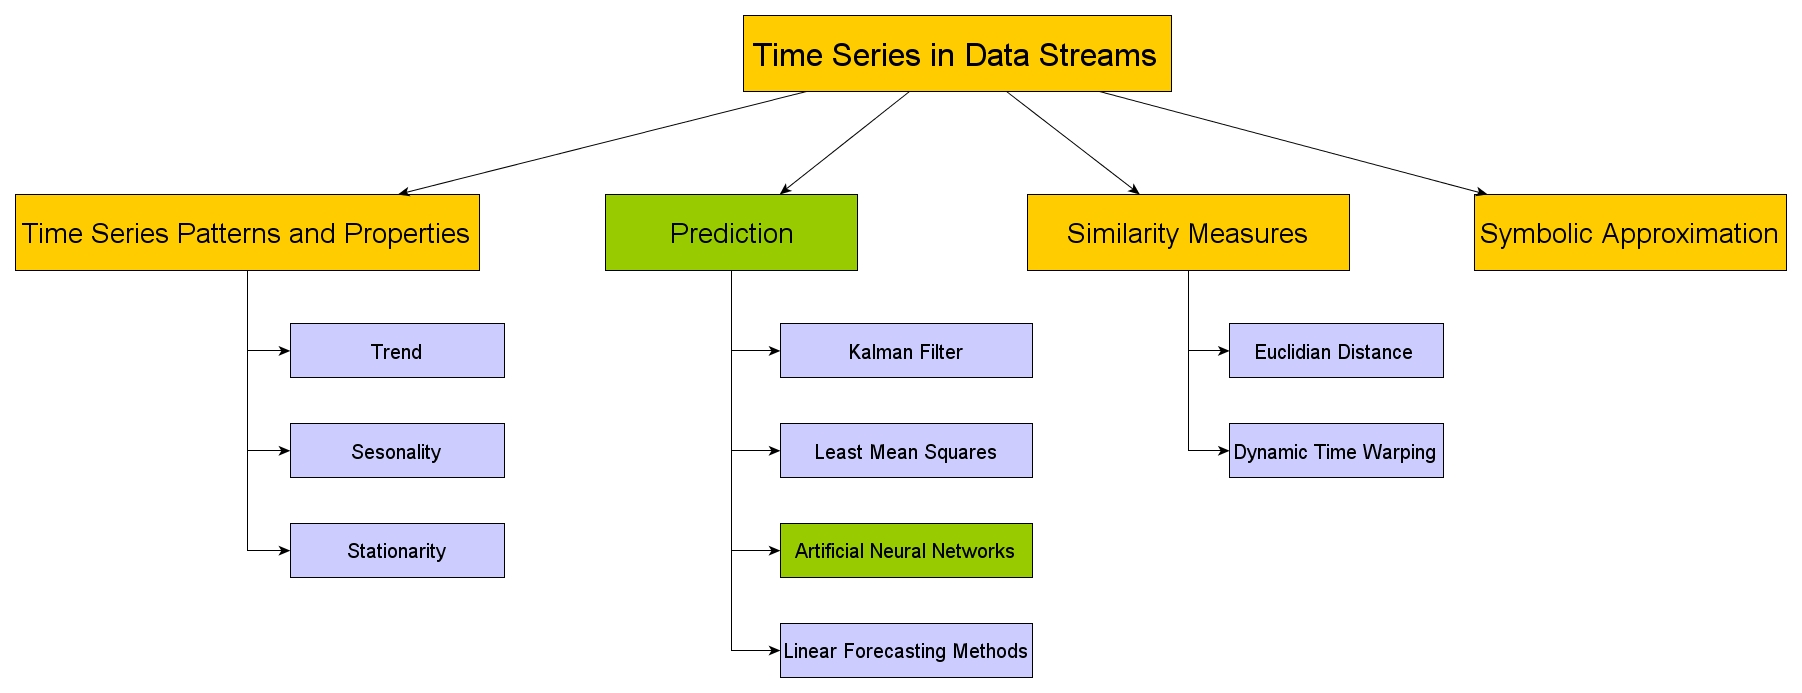
\includegraphics[width=\textwidth]{timeSeriesInDataStreamsOverview}
	\caption{An overview over the different research areas in time series analysis in data streams. The subcategories that are marked green are the categories, which are of interest in thesis and thus will be looked at more closely.}
	\label{fig_timeSeriesInDataStreamsOverview}
\end{figure}

Note that the research area of time series analysis is large and therefore there ae probably important subareas that are not mentioned by the author. We briefly go over the different areas that are not particularly relevant to this thesis:

\begin{itemize}
	\item \textbf{Time Series Patterns and Properties:} A lot of time series can be categorized according to their behavior and can be said to have certain properties. Among these are for example long term trends, seasonality (cyclic behavior) and stationarity ( mean, variance and autocorrelation are constant).
	\item \textbf{Time Series Similarity Measures:} Similarity of time series has many applications and can for example be used in k-NN classification. There are different similarity measures, which each have their advantages and disadvantages. Two well knowne examples are the classic euclidian distance and the dynamic time warping algorithm.
	\item \textbf{Symbolic Approximation:} Symbolic Approximation is a technique that aims to discretize time series into a string of arbitrary length. It can be of interest if one wants to apply algorithms that work on strings or categorical data on time series.
\end{itemize}

As already mentioned time series prediction (also called forecasting) is relevant for this thesis due to the emprirical evaluation which uses financial time series data. Thus, instead of giving an overview over the general topic of time series prediction, we devote the next subsection to exclusively report the state of the art on the prediction of financial time series. Very broadly forecasting methods can be divided into linear and non-linear methods. Linear models are usually simpler, but are at a disadvantage when the underlying model is non-linear \cite{zhang2003time}. Non-linear methods, such as neural networks are more powerful, in fact it has been shown that neural networks can in theory model any non-linear function \cite{abraham2005artificial} \cite{funahashi1989approximate}. However, building and training an actual neural network is a difficult task, since multiple design choices (such as the number of hidden neurons, the activation function and the initial weights) need to be made, which usually requires expert knowledge of both the underlying domain as well as neural networks in general in order to train an appropriate network \cite{abraham2005artificial}. Researchers have also tried to combine both approaches in order to form hybrid methods \cite{zhang2003time}. \newline
Neural networks were originally conceived as batch methods, meaning there were used in an offline scenario with no new data coming in constantly. However adapting them to the stream environment is surprisingly simple in most cases and has been done on multiple occasions \cite{chang2002real} \cite{frank2001time}. In fact, the streaming environment can be beneficial to neural networ training, since training a neural network in a static environment usually means making multiple passes over the training data, due to the lack of training data. If done incorrectly this can result in overlearning the training data and thus poor generalization. In the streaming environment however, there is an abundance of data, which means that each example has to be processed only once \cite{gama2010knowledge}. \newline
Predicting or forecasting time series values is normally very domain specific which results in different domains having their own specialized forecasting methods or specific modifications of popular general predictive models. Some of the domains in which time series forecasting is relevant are:

\begin{itemize}
	\item Stock market prediction (see subsection TODO for a detailed review of the state of the art)
	\item Electricity demand forecasting 
	\item Solar energy forecasting (TODO: better phrase
\end{itemize}

TODO: mention papers of the above domains and maybe explain neural networks
%As already mentioned many data mining algorithms for data streams make compromises of some sort or employ appoximations. Especially in the area of pattern mining there are quite a few approaches that use approximations or focus on the most recent data. Gianella et. al. have for example developed an algorithm to incrementally maintain approximately frequent itemsets for the most recent time windows using tilted time window frames \cite{giannella2003mining}. Approaches to mine frequent items without tilting the time windows exist as well, such as the sticky sampling or the lossy counting algorithm \cite{manku2002approximate}. These algorithms can be generalized to mine frequent itemsets, too. If this is done however pruning the candidates may become an issue if the main memory is small (the number of candidates to maintain may be too large). \newline
%A paper also related to regression and time series forecasting was published by Papadimitriou et. al. \cite{papadimitriou2003adaptive}. The authors tackle the problem of cyclic time series mining, as well as time series prediction of numerical values in potentially infinite data streams. \newline
%The rise in popularity of mining data streams also pushes research areas like distributed data mining, in which parallelized versions of data mining algorithms are researched. Large data streams and distributed systems often go hand in hand, which creates the need for distributed algorithms. Such solutions have been researched for example for frequent pattern mining \cite{lin2015fast}, association rule mining \cite{ashrafi2004odam}, clustering \cite{januzaj2004dbdc} and classification (in this case a distributed boosting algorithm) \cite{lazarevic2001distributed}. \newline
%A slightly different direction to data stream processing is querying data streams. Some contributing data scientists have thus approached streams in a similar manner as relational databases \cite{motwani2003query}. The authors present their progress at building a general purpose Data Stream Management System (DSMS) prototype, as a pendant to the traditional Database Management Systems (DBMS). They suggest the usage of an extension of SQL as a stream query language to allow for continuous queries and discuss approximation techniques. 
%
%
%\subsection{Classification and Regression}
%\label{subsec_regression}
%
%Classification and regression are the main applications of supervised learning. They are very similar and closely interlinked to each other. Classification aims to assign new, unseen objects to a class based on a model that was created from training data. Class labels are categorical. Regression is similar, but instead of assigning categorical class labels to new data points it is now the goal to generate a numerical (real) value that is close to the actual value. 
%A comprehensive overview over most classification approaches was comprised by Kotsiantis et. al. \cite{kotsiantis2007supervised}. The authors distinguish between different types of classifiers:
%\begin{itemize}
%	\item logical classifiers such as Decision Trees and rule based algorithms
%	\item preceptron based classifiers, such as the single layered perceptron or artificial neural networks
%	\item statistical classifiers, such as naive bayes or bayesian networks
%	\item instance based classifiers, such as k nearest neighbor
%	\item maximum margin classifiers, such as support vector machines
%\end{itemize}
%It is notable that the authors do not mention ensemble learners \cite{dietterich2000ensemble}, which combine several classifiers and classify new examples by letting each classifier vote. Arguably the most notable ensemble learning technique is the random forest \cite{liaw2002classification}.
%It is important to keep in mind that most classification approaches can also be tweaked to do regression, a random forest for instance can either be used to estimate a (binary) class label (classification) or a numerical value (regression).
%Classification and regression have also been attempted by using pattern mining and association rule generation \cite{ma1998integrating}. Instead of mining all association rules the authors focus on finding so called class association rules. An especially relevant application of rule based regression was the usage of classification rules using minimal rule generation for the prediction of equity returns \cite{apte1994predicting}. The authors modify a classification rule generation technique called R-MINI to be able to do regression. They evaluate their approach on historical stock market data from the S\&P 500 data-set (data is aggregated to monthly values). 
%While both of these pieces of work are interesting and extremely relevant to the problem tackled by this thesis it is important to note that they were both done in 1998 and 1994 respectively, so it is expected that the state of the art has changed since then.



%\subsection{Complex Event Processing and Episode Mining}
%\label{subsec_eventProcessing}
%Before talking about the state of the art in complex event processing it is first important to clarify the term \textit{"event"} which is a is very broad term that is used in many different areas of science. Even when restricted to computer science there may be different definitions with subtle differences. As already explained in the introduction this thesis will focus on events as defined by the glossary of the event processing society \cite{luckham2011epts}.
%When talking about processing complex events there is an important difference between two cases:
%
%\begin{itemize}
%	\item The patterns of interest are known before looking at the data. This is called complex event detection.
%	\item There is no prior knowledge about which patterns might be interesting, they need to be discovered while looking at the data. This is called complex event discovery or complex event mining (which basically means that data mining methods need to be employed)
%\end{itemize}
%
%Complex event detection usually revolves around specification and query languages for complex events \cite{eckert2009complex}. Quite a few different specification and query languages have been developed, such as SNOOP \cite{chakravarthy1994snoop} or the SASE event processing language \cite{wu2006high}. \newline
%Discovering interesting complex events of arbitrary structure in data streams is a very challenging task, thus most work focuses on specific types of complex events. A popular example is mining frequent sequences of events (basically complex events that only use the sequence operator) \cite{bettini1998mining} \cite{hasan2015probabilistic}. \newline
%This thesis deals with a more expressive type of complex events: Episodes. Originally episodes were researched without any relation to event processing \cite{mannila1995discovering}. 
%Episodes have roughly been categorized as serial, parrallel or composite and there are different mining methods proposed for each of these \cite{mannila1995discovering} \cite{zhou2010mining}. The connection between episodes and hidden markov models was also explored in a PHD thesis by Laxman \cite{laxman2006discovering}.
%Evaluating episode mining algorithms on real-life datasets is often difficult due to a lack of knowledge about the ground truth. Thus, generation of realistic, synthetic datasets has been looked into as well \cite{zimmermann2012generating}.

\subsection{Semantic Web}
\label{subsec_semanticWeb}
TODO



\section{Stock Market Forecasting}
\label{sec_prediction}
When reviewing the related work for te forecasting of stock markets, it is important to note that in a lot of cases, financial time series are not analyzed in a streaming environment. Authors commonly attempt to forecast daily closing values of stock markets, which means that in this case data velocity is very low (one new data point per day). However many techniques applied in these scenarios can also be applied in more rapidly moving streams. Examples of these are autoregressive models (TODO cite example) or artificial neural networks \cite{gama2010knowledge}. \newline
A good starting point into the prediction of stock market movements is provided by a literature study by Atsalakis et. al. \cite{atsalakis2009surveying}. The authors review more than 100 papers that attempt to predict stocks or stock indices. Figure \ref{fig_financialTimeSeriesPredictionOverview} visualizes some of the different properties and experimental settings of the approaches covered by Atsalakis et. al. (TODO: better phrase)

\begin{figure}[h]
	\centering
  	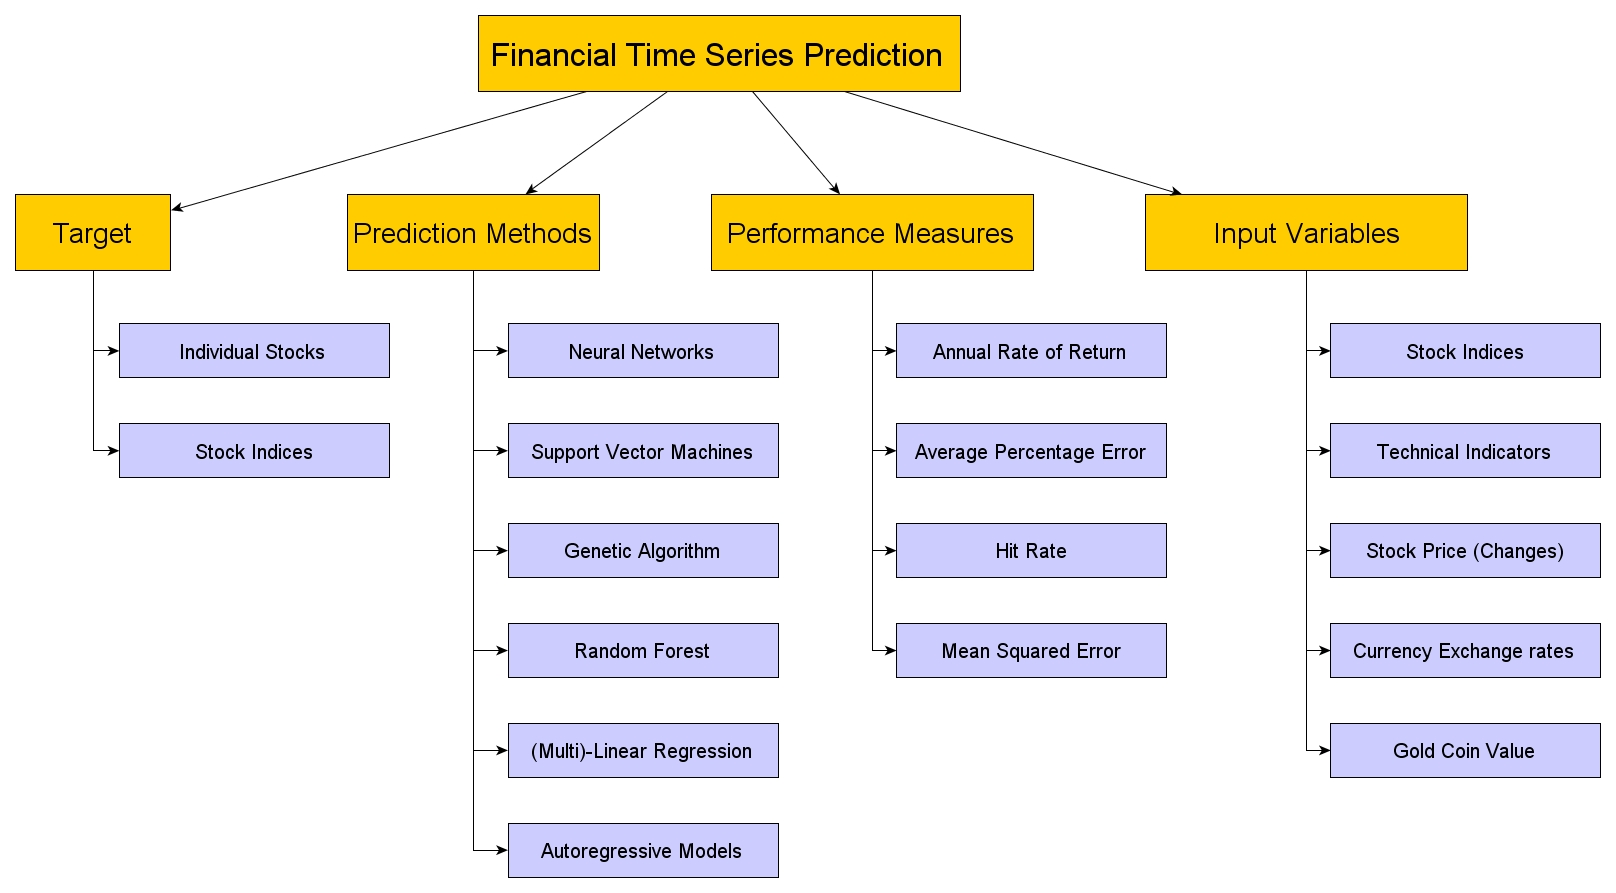
\includegraphics[width=\textwidth]{financialTimeSeriesPredictionOverview}
	\caption{An overview over different properties, experimental settings and approaches to the forecasting of of stock markets}
	\label{fig_financialTimeSeriesPredictionOverview}
\end{figure}

Most of the visualized information in figure \ref{fig_financialTimeSeriesPredictionOverview} was taken from the previously mentioned literature study by Atsalakis et. al. \cite{atsalakis2009surveying}. However  some pieces of work were not covered in that study such as (TODO: cite random forest /autoregressive models). We briefly review the different properties and categories visualized in figure 
\ref{fig_financialTimeSeriesPredictionOverview}:

\begin{itemize}
	\item \textbf{Target:} The target that is to predict can in theory be any financial index, indicator or price of interst. Many researchers tried to forecast the movement of stock indices (TODO: cite a bunch). However, also individual stocks have received attention (TODO: cite). TODO: more (if yes, then also more in figure) 
	\item \textbf{Performance Measures:} When building models it is crucial to measure their performance to enable comparison to other models. The number of different performance measures in this case is surprisngly large and diverse. The employed measures range from economic measures, such as the annual rate of return or the Hit-Rate to more technical measures such as the average percentage error or the mean squared error to only name a few (TODO: include more in figure?) . It is impractical to visualize or enumerate all measures that are in use, thus we limit ourselves to the previous examples. For a comprehensive list we refer the reader to the literature study by Atsalakis et. al. \cite{atsalakis2009surveying}.
	\item \textbf{Input Variables:} In real world scenarios this is probably the most important category. No matter which kind of elaborate model is built, if the choice of the input variables is poor, meaning they contain little information, then the model built from those simply can not perform well. This is especially true for financial time series, since those are known to be chaotic and noisy (TODO: cite). In fact there are reserachers that argue that financial time series follow the principle of random walks (TODO cite) which would imply that accurately, meaning better than random, forecasting financial time series is impossible. However there is a considerable amount of papers that suggest otherwise (TODO: cite). TODO: talk about input variables.
	\item \textbf{Prediction Methods:} While figure \ref{fig_financialTimeSeriesPredictionOverview} mentions many different approaches to the forecasting of stock markets, a large majority of the published papers in this area uses some form of neural network \cite{atsalakis2009surveying}. In fact Atsalakis et. al. note that 60\% of the papers they surveyed use feed forward Neural Networks and recurrent networks \cite{atsalakis2009surveying}. 
\end{itemize}


The literture study by Atsalakis et. al. reveals that the majority of the related work uses some form of neural network


%Similar to regression and classification, but not quite the same is prediction. Prediction (sometimes also called forecasting) introduces a new dimension, which is time. The task in prediction is to build a model that if given data points on a timeline will predict which data point will show up next.
%Due to its dependency on time, prediction plays a large role when mining time series data. Arguably the most popular models for time series prediction are artificial neural networks which are used by multiple authors with differnt variations and application domains \cite{connor1994recurrent} \cite{martinetz1993neural} \cite{frank2001time}. Of particular interest for this thesis are of course prediction approaches that were used in the same domain, namely stock market or financial time series prediction. Naturally this has been looked into. Gestel at. al. used support vector machines to predict the closing values of stock market indices \cite{van2001financial}.% (TODO: Talk/Read more about this paper, the bayesian networks, that are used too) 
%Another, more recent approach used an artificial neural network with an improved learning algorithm (by integrating improved bacterial chemotaxis optimization into the back propagation of the neural network) to successfully predict the Standard’s \& Poor’s 500 index (changes were aggregated to daily values).
%Another different approach is to use grey system models to predict time series \citep{kayacan2010grey}, in this specific case the authors predict the daily foreign currency exchange rate of euro to dollar. A comprehensive comparison of different models for predicting the S\&P CNX NIFTY index was carried out by kumar et. al. \citep{kumar2006forecasting}. The best performing model in their study is the support vector machine, closely followed by a random forest. This is interesting, since random forests have not received as much attention for time series prediction as for example artificial neural networks. Of course no general conclusions can be drawn from the performance of these models for one index. An very detailed overview over a lot of work in the area can be found in the literature study done by Atsalakis et al. \cite{atsalakis2009surveying} although the focus seems to be on papers that use neural networks or support vector machines.
%The attentive reader will have noticed that most of the previously named examples focus on predicting stock indices, a.k.a the general direction of the market. Predicting individual stock values has been looked at less, but there is of source some previous work to be considered. For example mahfoud et. al. compare genetic algorithms to neural networks for the prediction of individual stocks \cite{mahfoud1996financial}.





\section{Episodes}
\label{sec_episodes}
This section gives a detailed introduction to the topic of episode mining and presents an overview over the most relevant related work.

\subsection{Basic Definitions}

As already mentioned, episodes are complex events whose basic building blocks are simple events. Note that  in order to make use of episodes we require that all simple events have a type and we have a finite, previously known event alphabet, that contains these types, which we refer to as $\Sigma$. We follow up with a formal definition:

\begin{mydef}
\textbf{Episode} An episode (also sometimes called episode pattern or elementary episode) $\alpha$ of length $m$ (also called m-episode) is defined as a triple: $\alpha = (V_\alpha,{\leq}_{\alpha},g_\alpha)$ where $V_\alpha = \{v_1,...,v_m\}$ is a set of nodes, ${\leq}_{\alpha}$ is a partial order over $V_\alpha$ and $g_\alpha : V_\alpha \rightarrow \Sigma$ is a mapping that maps each node of $V_\alpha$ to an event type \cite{mannila1995discovering}.
\end{mydef}

Put more simply an episode is a multiset of event types, whose elements can be, but do not have to be ordered by a relation (${\leq}_{\alpha}$). Another way of putting it is that an episode is essentially a partially ordered sequence of events. Before we look at examples there are a two special types of episodes that need to be mentioned since they have received the most attention in the available literature. These are called serial and parallel episodes:

\begin{mydef}
\textbf{Serial Episode} An episode $\alpha = (V_\alpha,{\leq}_{\alpha},g_\alpha)$ is called a serial episode if ${\leq}_{\alpha}$ is a total order \cite{mannila1995discovering}.
\end{mydef}

\begin{mydef}
\textbf{Parallel Episode} An episode $\alpha = (V_\alpha,{\leq}_{\alpha},g_\alpha)$ is called a parallel episode if ${\leq}_{\alpha} = \emptyset$, in other words if there is no ordering imposed on $V_\alpha$ at all \cite{mannila1995discovering}.
\end{mydef}

Essentially, serial episodes are sequences, while parallel episodes are multisets. Figure \ref{fig_exampleEpisodes} visualizes example episodes as directed acyclic graphs (DACs), which is a useful way to visualize episodes. 


\begin{figure}[H]
\centering
\begin{tabular}{c|c|c}
\begin{subfigure}{.3\textwidth}
  \centering
  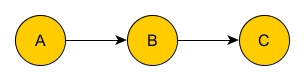
\includegraphics[width=\linewidth]{exampleSerialEpisode}
  \caption{A serial episode}
  \label{fig:sub1}
\end{subfigure}%
&
\begin{subfigure}{.3\textwidth}
  \centering
  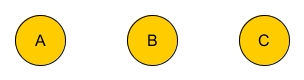
\includegraphics[width=\linewidth]{exampleParallelEpisode}
  \caption{A parallel episode}
  \label{fig:sub2}
\end{subfigure}
&
\begin{subfigure}{.3\textwidth}
  \centering
  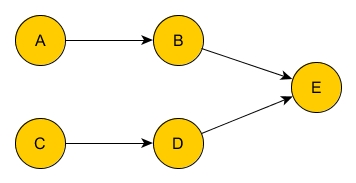
\includegraphics[width=\linewidth]{exampleCompositeEpisode}
  \caption{An elementary (composite) episode}
  \label{fig:sub3}
\end{subfigure}
\end{tabular}
\caption{Different example episodes visualized as directed acyclic graphs}
\label{fig_exampleEpisodes}

\end{figure}

In fact each episode can be formally transformed to a DAC using the following simple procedure: Given an Episode $\alpha = (V_\alpha,{\leq}_{\alpha},g_\alpha)$, create the corresponding DAC $G = (V,E)$ by executing the following:

\begin{enumerate}
	\item For each $v \in V_\alpha$ add $v$ to $V$ and label $v$ with $g_\alpha (v)$
	\item For each pair $v,w \in V_\alpha$ where $v \, {\leq}_{\alpha} \, w $ add edge $(v,w)$ to $E$
\end{enumerate}

The original paper by Manilla et.al. \cite{mannila1995discovering} also introduces the notion of composite episodes. We repeat the definition here:

\begin{mydef}
\label{def_compositeEpisodes}
\textbf{Composite Episode} An episode $\alpha = (V_\alpha,{\leq}_{\alpha},g_\alpha)$ is called a composite episode if $g_\alpha : V_\alpha \rightarrow \Sigma \cup C^*$, where $C^*$ is the set of all composite episodes.
\end{mydef}

This recursive definition of composite episodes may be confusing at first but it has the advantage that any elementary episode can be represented as a composite episode which is exclusively a serial or parallel composition of serial, parallel or composite subepisodes (see definition \ref{def_subEpisode}). \newline
Interestingly, there are other parts of the related work that use the term \textit{composite episodes} but deviate from definition \ref{def_compositeEpisodes}. For example Baathorn et. al. propose a method for finding composite episodes \cite{bathoorn2007finding}. However they define composite episodes as a sequence of parallel episodes, which is more restrictive than the original definition. Also Baumgarten et. al. use this definition \cite{baumgarten2003tree} when they present an approach to mine descriptive composite episodes. Note that not all elementary episodes can be represented as sequences of parallel episode. A simple example shown in figure \ref{fig_notSequenceOfSet} illustrates this. If the presented episode were to be represented as a sequence of parallel episodes obviously $A$ and $B$ would have to be in different parallel episodes in order to fulfill the requirement that $B$ must be after $C$. After that the problem is that it is impossible to assign $C$ to any of those sets. If it gets assigned to the same parallel episode set as $A$ then this would prohibit $A$ and $B$ occurring first followed by $C$, which is allowed in the original definition. Likewise if $C$ gets assigned to the same parallel episode as $B$ then that eliminates the possibility of $C$ occurring before $A$ and $B$, which once again was allowed in the elementary episode. In this thesis we will stick to the original definition as presented in definition \ref{def_compositeEpisodes}. \newline

\begin{figure}[h]
	\centering
  	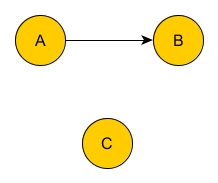
\includegraphics[width=0.3\textwidth]{notSequenceOfSet}
	\caption{An elementary episode that can not be represented as a sequence of parallel episodes}
	\label{fig_notSequenceOfSet}
\end{figure}

If we want to denote quick, simple episodes formally without drawing a DAC, we will use $\rightarrow$ as the sequence (ordering) operator. To show that there is no order specified between two nodes we use $\|$ as the parallel operator. For example $(A \, \| \, B ) \rightarrow C$ denotes a composite episode of length 3, which specifies that it does not matter in which order $A$ or $B$ occur, but $C$ must occur after both $A$ and $B$. If we want to discuss more complex episodes we will visualize them graphically like in the previous figures \newline  
The notion of sub- and superpatterns, which is very important for most pattern mining applications also applies to episodes, as shown in the next definition.

\begin{mydef}
\label{def_subEpisode}
\textbf{Subepisode} An episode $\beta = (V_\beta,{\leq}_{\beta},g_\beta)$ is said to be a subepisode of episode $\alpha = (V_\alpha,{\leq}_{\alpha},g_\alpha)$ if all of the following conditions hold:
\begin{enumerate}
	\item $V_\beta \subseteq V_\alpha$
	\item $\forall v \in V_\beta \; : \; g_{\beta}(v) = g_\alpha (v) $
	\item $\forall v,w \in V_\beta \, , v \, {\leq}_{\beta} \, w \; : \; v \, {\leq}_{\alpha} \, w$
\end{enumerate}
In this context we also refer to $\alpha$ as the superepisode of $\beta$ \cite{mannila1995discovering} \cite{laxman2007fast}.
\end{mydef}

It is important to note that in the original definition of sub- and superepisodes by Mannila et. al. \cite{mannila1995discovering}, the first property of the above definition was actually defined as $V_\beta \subset V_\alpha$, which implies that subepisodes would always have to consist of at least one less node than their superepisodes. This definition was changed by Laxman et. al. \cite{laxman2007fast} to allow set equality as well. The implications of this change are that parallel episodes like $A \| B$ are now subepisodes of their serial counterparts of the same length $A \rightarrow B$. In this thesis we stick to the definition that allows set equality between super- and subepisodes. \newline
It is helpful to think of episodes as a template or pattern for concrete occurrences. In order to define what we mean by an episode occurance, we first need to formally introduce the notion of an event sequence.

\begin{mydef}
\textbf{Event sequence} An event sequence is defined as an ordered list of tuples $S = [ (T_1,t_1),..., (T_n,t_n) ] $ where $T_i \in \Sigma$ is the event type of the i-th event and $t_i \in \mathbb{N}^+$ is the timestamp of the i-th event. The sequence is ordered according to the timestamps, which means that $\forall i,j \in {1,...,n} \; i<j \implies t_i \leq t_j$. %TODO: talk about time equality
\end{mydef}

\begin{mydef}
\label{def_episodeOccurrence}
\textbf{Episode Occurrence} An event episode $\alpha = (V_\alpha,{\leq}_{\alpha},g_\alpha)$ is said to occur in a sequence $S$ if events of the types that the nodes in $V_\alpha$ are mapped to by $g_\alpha$, occur in $S$ in the same order that they occur in the episode. More formally if we are given a sequence of events $S=[(T_1,t_1),...,(T_n,t_n)]$ we can define an occurrence of $\alpha$ as an injective Map $h:V_\alpha \rightarrow \{1,...,n\}$, where $g_\alpha (v) = T_{h(v)}$ and $\forall \, v,w \in V\alpha : v \;{\leq}_{E}\; w \implies t_{h(v)} \le t_{h(w)}$ holds \cite{mannila1995discovering}.
\end{mydef}

\subsection{Episode Detection and general Mining Algorithm}
When discovering episodes in a sequence one is usually interested in those episodes that occur frequently, meaning more often than a user defined threshold. This is similar to all the different kinds of pattern mining algorithms, such as the apriori algorithm for finding frequent itemsets \cite{agrawal1994fast}. A general algorithm for mining the episodes occurring frequently in a sequence is given in algorithm \ref{alg_generalEpisodeMining}. The algorithm is very alike the basic apriori algorithms, since it uses a level-wise, breadth first search by first identifying all frequent episodes of a certain length $i$ and then uses these frequent episodes to generate candidates (possibly frequent episodes) of length $i+1$. In order for this to be correct, episode frequency must follow the apriori principle \cite{agrawal1994fast}, which formally means that if an episode is frequent, all its subepisodes must be frequent as well. Intuitively one would assume that this is always true for episodes but strictly speaking this depends on the definition of episode frequency. However, any frequency definition of episodes that does not satisfy the apriori principle would be highly questionable to say the least, since this would eliminate the possibility of an efficient candidate generation that prunes those episodes which have infrequent subepisodes. To the best of our knowledge all frequency definitions proposed in the literature satisfy the apriori principle.\newline

\begin{algorithm}[H]
  \caption{General mining algorithm for frequent episodes
    \label{alg_generalEpisodeMining}}
  \begin{algorithmic}[1]
    \Statex
    \Function{EpisodeMining}{}
      \Let{$C_i$}{Episodes of Size 1} 
      \Let{$freq$}{$\emptyset$}
      \Let{$i$}{$1$}
      \While{$C_i \neq \emptyset$}
      	\State Count frequencies of each Episode $E \in C_i$
        \Let{$L_i$}{ $\{ E \mid E \in C_i \land C_i \; is\; frequent\}$}
        \Let{$freq$}{$freq \cup L_i$}
        \Let{$C_{i+1}$}{Generate Episode Candidates of length $i+1$ from $L_i$}
        \Let{$i$}{$i+1$}
      \EndWhile
      \State \Return{$freq$}
    \EndFunction
  \end{algorithmic}
\end{algorithm}


In summary, the general mining algorithm for frequent episodes requires:

\begin{itemize}
	\item A definition of episode frequency, that does not violate the apriori principle
	\item An algorithm for counting episode frequency (of concrete candidates) according to this definition
	\item An algorithm to generate candidate episodes
\end{itemize}

It may be a bit confusing that we need a definition of episode frequency for such a mining algorithm. Since we have already defined what an occurrence of an episode looks like it would seem that counting all occurrences of an episode would yield its frequency. While this is a possible definition of frequency, it is important to note that finding all occurrences of an episode within a sequence is neither practical nor useful. An example will demonstrate the problem with this. Consider the simple serial episode $A \rightarrow B$ and a sequence of length $2\cdot n$ which repeats the subsequence $(A,B)$ $n$ times. One quickly realizes that the number of episode occurrences is very large due to the possibility of overlapping episode occurrences. In this particular case there are already $ \frac{n \cdot (n+1)}{2}$ possible occurrences. This number swiftly increases with the size of the episode pattern, since it introduces more potential overlappings. Naturally the number of possible parallel and composite episode occurrences is even larger, since they are less restrictive in the order of the events. Additionally, such a frequency definition would violate the apriori principle, since subepisodes can have less occurrences than their superepisodes. Consider the example sequence $[A,B,C,A,B,C]$ (timestamp values are left out). In this sequence there are 3 distinct occurences for the episode $A \rightarrow B$ and four distinct occurrences for its superepisode $A \rightarrow B \rightarrow C$. These detrimental effects of this naive frequency definition are nicely summarized by Laxman et. al. in a paper presenting the non-overlapped frequency definition \cite{laxman2007fast}. \newline
This leads to various frequency definitions of episodes in the literature, which will be dealt with in subsections \ref{subsec_windowBased} and \ref{subsec_otherFrequency}. Each frequency definition comes with its own frequency counting algorithm. The procedure for generating candidates is independent of the frequency definition and is presented in \ref{subsec_candidateGen}. \newline
%The first two definitions, which we will refer to as window based frequency and minimal occurance based frequency, are mentioned by Zimmermann, when he presents his method for synthetic episode generation \cite{zimmermann2012generating}, but were originally conceived in (TODO: include original sources). We refer to the third definition as the non-overlapping occurrence based Frequency which was suggested by Laxman et al. \cite{laxman2007fast}.


\subsection{Window based frequency}
\label{subsec_windowBased}
To the best of our knowledge the window based frequency was the first frequency definition for episodes to gain general popularity. It was conceived by Mannila et. al. \cite{mannila1995discovering}, although the frequency counting algorithms were only mentioned in text form. The same authors  specified the algorithms in a later paper \cite{mannila1997discovery}, which acts as the primary source for the overview given in this subsection. In order to define the window based frequency we first need the notion of a time window: 

\begin{mydef}
\textbf{Time Window} Given a sequence of events $S$ we define the Time Window $W(S,q,r)$ with $q,r \in \mathbb{N}^+$ and $q < r$ as the ordered subsequence of $S$ that includes all events of the annotated event stream $S$ that have a timestamp $t$ where $q \leq t\leq r$. We call $w = r-q+1$ the size of Window $W$.
\end{mydef}

%TODO: nice picture visualizing the different windows 

\begin{mydef}
\textbf{Episode Frequency - Window based Definition} Given a sequence of events $S$, a fixed window size of $w$ and an episode $\alpha$, we define the window based frequency $w\_freq(\alpha )$ as the number of windows $W$ with size $w$ of $S$ in which $\alpha$ occurs: $w\_freq(\alpha ) = |\,\{W(S,q,r) \mid r-q+1 = w \land \alpha \;occurs\; in\; W \}\,|$. %TODO: incorporate sequence bounds and number of windows
\end{mydef}

For example given a sequence $S = [ (12,A) , (14,B) , (19,C) , (22,A), (34,D) ]$ the Episode $\alpha = B \rightarrow A$ occurs in window $W(S,14,22)$. \newline 
This definition can be confusing at first since it is intended that episode occurrences that are comprised of the exact same events count just as many times as there are windows in which the events appear. If we have a window size of $w=11$ for the previously mentioned example, we can find the episode $B \rightarrow A$ in the consecutive windows $W(S,12,22)$, $W(S,13,23)$ and $W(S,14,24)$, which means we will get a frequency of $3$ just for the two events $(14,B)$ and $(22,A)$. This effect obviously increases with the window size. Note that for each episode $\alpha$ we only count one occurrence per window $W$, no matter how many occurrences of $\alpha$ there are in $W$.\newline
When determining the window based frequency the naive approach would be to check each window of the sequence separately. Since the windows are adjacent there is a better approach, which makes it possible to only iterate over the sequence once and determine the window based frequency for each candidate episode. Most papers focus purely on parallel and serial episodes and do not give an algorithm for composite episodes. The algorithms to determine the window based frequency of serial and parallel episodes are given in algorithm \ref{alg_windowBasedParallel} and \ref{alg_windowBasedSerial} respectively. The basic ideas are described below. \newline \newline

\textbf{Frequency Counting of parallel Episodes} \newline
The algorithm for counting the frequency of parallel episodes uses the following data structures and variables:

\begin{itemize}
	\item For each event type $A$ store the number of occurrences of this event in the current window in $A.count$
	\item For each episode $\alpha$ store 
	\begin{itemize}
		\item $\alpha .freq$ - the number of windows in which alpha occurred so far
		\item $\alpha. eventCount$ - the number of events of $alpha$ that are present in the current window
		\item $\alpha. inwindow$ - this variable gets set to the current time whenever $\alpha$ becomes fully present ($alpha .eventCount = |\alpha |$).
	\end{itemize}
	\item additionally maintain $contains$ which is a set of sets. Each set in $contains$ is identified by a tuple $(T,i)$, where $T \in \Sigma$ is an event type and $i \in \mathbb{N}^+$. These sets are referred to as $contains(T,n)$. The set $contains(T,n)$ contains all candidate parallel episodes, which contain the event type $T$ exactly $n$ times. This is done to be able to efficiently access candidates, when certain events enter or leave the window.
\end{itemize}

The algorithm works as follows. First the above mentioned variables and index structures are initialized. Subsequently we perform the main loop which iterates through every point of time between the start and the end time of the sequence (TODO: they start earlier for some reason?). Essentially each iteration is sliding the window one step forwards. The only two things that need to be handled inside the loop are new events coming into the window and old events dropping out of the sliding window. If a new event comes in its count gets updated and each episode $\alpha$ that is affected by this will get its event count updated and, if it is completed, the current time will be saved in $\alpha. inwindow$. \newline
If an event $A$ drops out of the window, for all episodes $\alpha$ that occurred in the previous window(s) and now no longer have an occurrence in the current window (by losing $A$) the number of windows they were present in gets added to $\alpha .freq$.

\begin{algorithm}[H]
  \caption{Calculate Window based Frequency for parallel Episodes
    \label{alg_windowBasedParallel}}
  \begin{algorithmic}[1]
    \Statex
    \Require Let $C$ be the set of candidate parallel episodes, and let $S=[(T_1,t_s),...,(T_n,t_e)]$ be a sequence of events, let $win$ be the window size and finally let $minS$ be the minimum support.
      \State \textit{// Initialization}
      \For{each $\alpha \in C$}
      	\For{each $A \in \alpha$}
      		\Let{$A.count$}{$0$}
      		\For{$i \in \{1,...,|\alpha |\}$}
      			\Let{$contains(A,i)$}{$\emptyset$}
      		\EndFor
      	\EndFor
      \EndFor
      \For{each $\alpha \in C$}
      	\For{each $A \in \alpha$}
      		\Let{$a$}{number of events of type $A$ in $\alpha$}
      		\Let{$contains(A,a)$}{$contains(A,a) \cup \{\alpha \}$}
      	\EndFor
      	\Let{$\alpha .eventCount$}{$0$}
      	\Let{$\alpha .freq$}{$0$}
      \EndFor
      \State \textit{// Recognition}
      \For{$start \gets t_s - win +1 \textrm{ to } t_e$}
      	\State \textit{//Bring new events to the window}
      	\For{each $(t,A) \in S $ where $t = start+win-1$}
      		\Let{$A.count$}{$A.count +1$}
      		\For{each $\alpha \in contains(A,A.count)$}
      			\Let{$\alpha .eventCount$}{$\alpha .eventCount + A.count$}
      			\If{$\alpha .eventCount = |\alpha | $}
          			\Let{$\alpha .inwindow$}{$start$}
       			\EndIf
      		\EndFor
 		\EndFor
 		\State \textit{// Drop old events out of the window}
 		\For{each $(t,A) \in S $ where $t = start-1$}
 			\For{each $\alpha \in contains(A,A.count)$}
 				\If{$\alpha .eventCount = |\alpha | $}
          			\Let{$\alpha .freq$}{$\alpha .freq + \alpha .inwindow -start $}
       			\EndIf
       			\Let{$\alpha .eventCount$}{$\alpha .eventCount - A.count$}
 			\EndFor
 			\Let{$A.count$}{$A.count -1$}
 		\EndFor
      \EndFor
      %\Let{$freq$}{$\emptyset$}
      %\Let{$i$}{$1$}
      %\While{$C_i \neq \emptyset$}
      	%\State Count frequencies of each Episode $E \in C_i$
       % \Let{$L_i$}{ $\{ E \mid E \in C_i \land C_i \; is\; frequent\}$}
       % \Let{$freq$}{$freq \cup L_i$}
       % \Let{$C_{i+1}$}{Generate Episode Candidates of length $i+1$ from $L_i$}
        %\Let{$i$}{$i+1$}
      %\EndWhile
      \State \Return{$\{\alpha \mid \alpha \in C \land \frac{\alpha.freq}{t_e - t_s + win -1} \geq minS\}$}
  \end{algorithmic}
\end{algorithm}

\textbf{Frequency Counting of serial Episodes} \newline
The basic idea when determining the window based frequency of serial episodes is that a serial episodes can be recognized by using automaton that accepts the events of its corresponding serial episode in exactly the specified order and ignores all other input. For each serial episode $\alpha$ there can be several instances of the recognizing automaton (in different states) at the same time. This is necessary in order to replace old occurrences with newer ones whenever possible. The algorithm for counting the frequency of serial episodes uses the following data structures and variables: %TODO figure visualizing automata

\begin{itemize}
	 \item Each episode $\alpha$ is represented as an array in which the event types contained in $\alpha$ are stored in the correct order
	\item For each episode $\alpha$ the number of windows in which alpha occurred so far is stored in $\alpha .freq$
	\item An automaton is simply represented by a tuple $(\alpha ,i)$, where $\alpha$ is the corresponding candidate serial episode and $i \in \{1,...,|\alpha |\}$ is the state (position in the episode) in which the automaton currently is.
	\item The automata are grouped by the event type that will allow them to perform the next transition. These lists are referred to as $waits(T)$, where $T \in \Sigma$ is an event type.
	\item For each automata belonging to episode $\alpha$ that is currently in state $i$, the time at which it this automaton was initialized is stored in $\alpha .initialized[i]$.
	\item Additionally any automata that were initialized at point of time $t$ will be contained in a list referred to as $beginsat(t)$.
	\item transitions to be made are stored in a list named transitions and are stored in the form $(\alpha ,i,t)$, where $\alpha$ is the corresponding episode, $i$ is the index of the state from which the automaton will transition to the next one and $t$ is the time in which this automaton was initialized.
\end{itemize}

The structure of the algorithm is the same as the one of algorithm \ref{alg_windowBasedParallel}. First the variables are initialized, then the sequence is looped over and the sliding window moves by one time unit in each iteration. A new instance of an automaton is initialized, whenever an event $A$ is the first event of an episode and enters the window. Additionally all automata that wait for $A$ will be moved to the next state, while memorizing their initial starting time. If an automaton of episode $\alpha$ moves to a state which is already occupied by another automaton, the old automaton is discarded (since the newer one has a later starting time and thus will be present in more windows). If an automaton reaches its final state the current time is memorized in $\alpha .inwindow$. If an automaton in its final state expires (its starting time drops out of the window) the number of windows it was present in is added to its corresponding sequence.


\begin{algorithm}[H]
	\caption{Calculate Window based Frequency for serial Episodes
    \label{alg_windowBasedSerial}}
  	\begin{algorithmic}[1]
    	\Statex
    	\Require Let $C$ be the set of candidate serial episodes, and let $S=[(T_1,t_s),...,(T_n,t_e)]$ be a sequence of events, let $win$ be the window size and finally let $minS$ be the minimum support. TODO: part of the algorithm is cut off
      	\State \textit{// Initialization}
      	\For{each $\alpha \in C$}
      		\For{$i \in \{1,...,|\alpha |\}$}
      			\Let{$\alpha .initialized[i]$}{$0$}
      			\Let{$waits(\alpha [i])$}{$\emptyset$}
      		\EndFor
      	\EndFor
      	\For{each $\alpha \in C$}
      		\Let{$waits(\alpha [1])$}{$waits(\alpha [1]) \cup \{(\alpha ,1)\}$}
      		\Let{$\alpha .freq$}{$0$}
      	\EndFor
      	\For{$i \in \{t_s -win,...,t_s -1\}$}
      		\Let{$beginsat(t)$}{$\emptyset$}
      	\EndFor
      	\State \textit{// Recognition}
     	\For{$start \gets t_s - win +1 \textrm{ to } t_e$}
     		\State \textit{//Bring new events to the window}
	    	\Let{$beginsat(start +win -1)$}{$\emptyset$}  
      		\Let{$transitions$}{$\emptyset$}
			\For{each $(t,A) \in S $ where $t = start+win-1$}
				\For{each $(\alpha ,j) \in waits(A)$}
					\If{$j = |\alpha | \land  \alpha .initialized[j] = 0$}
          				\Let{$\alpha .inwindow$}{$start$}
       				\EndIf
       				\If{$j = 1$}
       					\Let{$transitions$}{$transitions \cup \{(\alpha ,1, start+win-1 \}$}
       				\Else
       					\Let{$transitions$}{$transitions \cup \{(\alpha ,j, initialized[j-1]) \}$}
						\State Remove $(\alpha, j-1)$ from $beginsat(\alpha .initialized[j-1])$
						\Let{$\alpha .initialized[j-1]$}{$0$}
						\State Remove $(\alpha, j)$ from $waits(A)$
       				\EndIf	
       			\EndFor
			\EndFor      		
      		\For{each $(\alpha ,j,t) \in transitions$}
      			\Let{$\alpha .initialized[j]$}{$t$}
      			\Let{$beginsat(t)$}{$beginsat(t) \cup \{(\alpha ,j)\}$}
      			\If{$j \le |\alpha |$}
      				\Let{$waits(\alpha [j+1])$}{$waits(\alpha [j+1]) \cup \{(\alpha , j+1)\}$}
      			\EndIf
      		\EndFor
      		\State \textit{// Drop old events out of the window}
      		\For{each $(\alpha ,l) \in beginsat(start-1)$}
      			\If{$l = |\alpha |$}
      				\Let{$\alpha .freq$}{$\alpha .freq + start - \alpha .inwindow$}
				\Else
					\State Remove $(\alpha, l+1)$ from $waits(\alpha [l+1])$      			
      				\Let{$\alpha .initialized[l]$}{$0$}
      			\EndIf
      		\EndFor
      	\EndFor
      	\State \Return{$\{\alpha \mid \alpha \in C \land \frac{\alpha.freq}{t_e - t_s + win -1} \geq minS\}$}
  \end{algorithmic}
\end{algorithm}

%TODO: discuss complexity \newline

Naturally there are enhancements to these algorithms. For example both counting algorithms iterate over each point of time $t$ between the start and end time of the sequence, regardless of the fact that there might not be anything to do at this point of time (no event drops out of the window and no new event comes in). Especially if the sequence of events is sparse, meaning that the time between events is usually large, this will become problematic. This issue can be fixed rather easily: instead of increasing $start$ by one in each iteration, one can increase start by the amount of time that is needed until a change in the window occurs and update the data structures accordingly. \newline
There is a notable absence of frequency counting algorithms for elementary (composite) episodes in literature. Mannila et. al. claim that each composite episode can be broken down into partial episodes, which are serial and/or parallel \cite{mannila1997discovery}. However they neither specify an algorithm for breaking down composite episodes into purely serial and parallel parts, nor do they specify a frequency counting algorithm for composite episodes. Subsequent research, such as alternate frequency definitions and counting algorithms has also mainly focused on parallel and serial episodes. If composite episodes have been studied they were usually studied in the above mentioned, more restrictive form of sequences of parallel episodes. \newline

\subsection{Other frequency definitions}
\label{subsec_otherFrequency}

In this subsection we briefly present alternative frequency definitions. However we do not present the respective counting algorithms, since they are not as relevant for this thesis. For the exact algorithms we refer the reader to the respective papers. \newline
Most alternative definitions tried to move away from the ideas of fixed windows and tried to improve the performance of the counting algorithms. \newline \newline

\textbf{Minimal Occurrence Based Frequency Definition} \newline
The first alternate definition does uses the concept of minimal occurrences:

\begin{mydef}
\textbf{Minimal Occurrence} An event episode $\alpha$ is said to occur minimally in a window $W(S,q,r)$ if $\alpha$ occurs in $W$ and there is no subwindow of $W$ in which $\alpha$ also occurs. %(TODO: define subwindow)
\end{mydef}

\begin{mydef}
\textbf{Episode Frequency - Minimal Occurrence based Definition} Given a sequence of events $S$ and an Episode $\alpha$, we define the minimal occurrence based frequency $mo\_freq(\alpha )$ as the number of minimal occurrences of $\alpha$ in $S$. TODO: find and cite the original source
\end{mydef}

The second alternative definition introduces the concept of non-overlapping occurrences:

\begin{mydef}
\textbf{Non-Overlapping Occurrences} Given a m-Episode $\alpha = (V_\alpha,{\leq}_{\alpha},g_\alpha)$ where $V_\alpha = \{v_1,...,v_m\}$, two occurrences $h_1$ and $h_2$ of $\alpha$ are non-overlapped if either 
\begin{itemize}
	\item $\forall \, v_j \in V_\alpha : h_2(v_1)>h_1(v_j)$ or 
	\item $\forall \, v_j \in V_\alpha : h_1(v_1)>h_2(v_j)$
\end{itemize}
A set of occurrences is non-overlapping if every pair of occurrences in it is non-overlapped \cite{laxman2007fast}.
\end{mydef}

This leads to the Definition:

\begin{mydef}
\textbf{Episode Frequency - Non-Overlapping Occurrences based Definition} Given a seqeunce of events $S$ and an Episode $\alpha$, we define the non-overlapping occurrence based frequency $noo\_freq(\alpha )$ as cardinality of the largest set of non-overlapped occurrences of $\alpha$ in $S$ \cite{laxman2007fast}.
\end{mydef}

When looking at these definitions in comparison to the window based frequency definition it is not clear whether any of these is always superior to or more useful than the other since they have different properties. We mention them briefly:

\begin{itemize}
	\item As already mentioned the window based frequency counts an episode occurrence that is comprised of the same events in multiple windows. This might especially distort the count if the window size is high and the events in the episode happen with minimal delay between them.
	\item The minimal occurrence based definition of frequency does not suffer from the problem of the previous point
	\item The window based definition has the advantage that it already incorporates a fixed size during which episodes may occur, meaning there can not be episodes that stretch over a time period larger than the fixed window size $w$. This might be beneficial for potential algorithms, since it reduces the search space for episodes. On top of that it is also closer to reality, since in many domains episodes happen within a small time window \cite{generatingEpisodeDatasets}.
	\item The non-overlapping occurrence based frequency offers the fastest counting algorithm of all three definitions. However when incorporating expiry times for serial episodes it looses this advantage. Additionally previous literature has not yet identified an efficient algorithm to count non-overlapped occurrences of parallel episodes with expiry times. 
\end{itemize}

\subsection{Candidate Generation}
\label{subsec_candidateGen}
Most previous work generates candidates for serial and parallel episodes separately, using a levelwise approach for both cases. The candidate generation procedure presented below was originally specified by Manila et. al. \cite{mannila1997discovery}. A more detailed explanation can be found in Laxman's PHD thesis \cite{laxman2006discovering}. \newline
We first consider the case for parallel episodes. Given $F_k$ as the set of all frequent parallel episodes of length $k$ we can generate the candidate parallel episodes $C_{k+1}$ of length $k+1$ by doing the following:

\begin{enumerate}
	\item Represent each candidate $\alpha \in F_k$ as a lexicographically sorted array of length $k$.
	\item For each unordered pair $(\alpha , \beta )$, $\alpha ,\beta \in F_k$ where $\alpha$ and $\beta$ share the same first $k-1$ nodes, generate candidate $\gamma$ by copying $\alpha$ and appending $\beta [k]$.
\end{enumerate}

For example the two frequent parallel episodes $A \| A \| B$ and $A \| A \| C$ will generate the candidate $A \| A \| C \| D$. \newline
The same procedure can be applied to serial episodes, except that
\begin{itemize}
	\item we do not order lexicographically, instead the serial episodes remain in the array in their natural order
	\item each pair $(\alpha , \beta )$ with the same properties as above now generates two candidates:
	\begin{itemize}
		\item $\gamma{_1}$ by copying $\alpha$ and appending $\beta [k]$.
		\item $\gamma{_2}$ by copying $\beta$ and appending $\alpha [k]$.
	\end{itemize}
\end{itemize}

Thus the two frequent serial episodes $A \rightarrow A \rightarrow B$ and $A \rightarrow A \rightarrow C$ will now generate the two candidates $A \rightarrow A \rightarrow B \rightarrow C$ and $A \rightarrow A \rightarrow C \rightarrow B$. \newline
Since the mining of composite episodes has not received much attention, it is unsurprising that there little related work that mentions candidate generation strategies for these general types of episodes (TODO: refer to later chapter, since I will do that). For a more strict definition of composite episodes which only includes sequences of parallel episodes, Baumgarten et. al. use a tree growth strategy to generate candidates for composite episodes \cite{baumgarten2003tree}. %TODO: expand this subsection if needed



%\section*{Subplots}
%I can cite Wall-E (see Fig.~\ref{fig:WallE}) and Minions in despicable me (Fig.~\ref{fig:Minnion}) or I can cite the whole figure as Fig.~\ref{fig:animations}


%\begin{figure}
%  \centering
%  \begin{subfigure}[b]{0.3\textwidth}
%   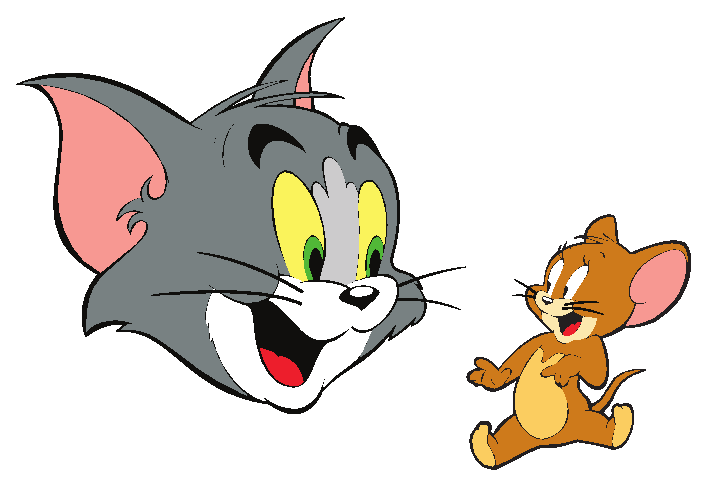
\includegraphics[width=\textwidth]{TomandJerry}
%  \caption{Tom and Jerry}
%    \label{fig:TomJerry}   
%  \end{subfigure}             
%  \begin{subfigure}[b]{0.3\textwidth}
%    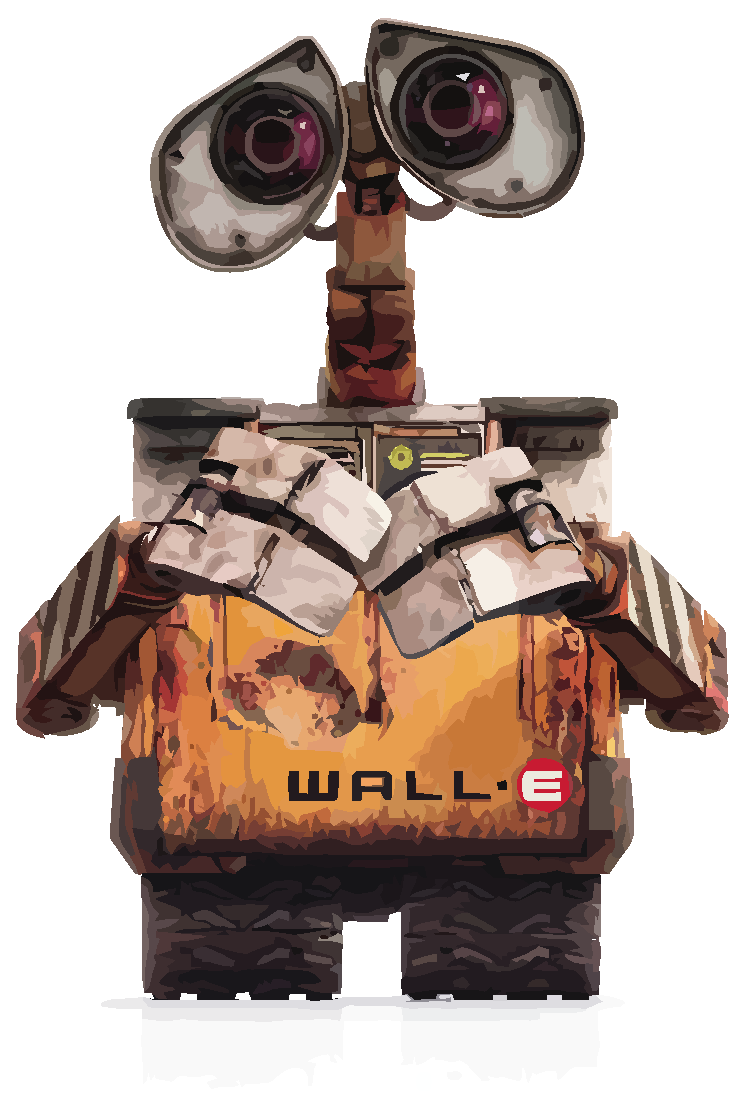
\includegraphics[width=\textwidth]{WallE}
%    \caption{Wall-E}
%    \label{fig:WallE}
%  \end{subfigure}             
%  \begin{subfigure}[b]{0.3\textwidth}
%    
\includegraphics[width=\textwidth]{minion}
%    \caption{Minions}
%    \label{fig:Minnion}
%  \end{subfigure}
%  \caption{Best Animations}
%  \label{fig:animations}
%\end{figure}


